\documentclass[12pt,a4paper]{report}
\usepackage[utf8]{inputenc}
\usepackage[T5]{fontenc}
\usepackage[vietnamese]{babel}
\usepackage{amsmath, amssymb}
\usepackage{graphicx}
\usepackage{geometry}
\usepackage{float}
\usepackage{hyperref}

% --- THƯ VIỆN ÉP KHOẢNG TRẮNG ---
\usepackage{titlesec}
% Giảm khoảng trắng khổng lồ mặc định của \chapter
\titleformat{\chapter}[display]
  {\normalfont\huge\bfseries}{\chaptertitlename\ \thechapter}{10pt}{\Huge}
\titlespacing*{\chapter}{0pt}{-25pt}{15pt} 
\titlespacing*{\section}{0pt}{10pt}{5pt}   
\titlespacing*{\subsection}{0pt}{10pt}{5pt} 

% Cấu hình margin
\geometry{a4paper, margin=2cm}

% Cấu hình link
\hypersetup{
    colorlinks=true,
    linkcolor=black,
    filecolor=magenta,      
    urlcolor=blue,
    pdftitle={Báo cáo Đề tài AI},
}

\begin{document}

% ================= TRANG BÌA =================
\begin{titlepage}
    \centering
    \vspace*{0.5cm}
    \Large \textbf{ĐẠI HỌC PHENIKAA} \\
    \Large \textbf{TRƯỜNG CÔNG NGHỆ THÔNG TIN PHENIKAA} \\
    \vspace{1.5cm}
    
\includegraphics[width=0.4\textwidth]{logoo.jpg} 
    \vspace{1.5cm} \\
    \Large \textbf{TÊN HỌC PHẦN: NHẬP MÔN TRÍ TUỆ NHÂN TẠO} \\
    \vspace{0.5cm}
    \Large \textbf{TÊN ĐỀ TÀI: CÀI ĐẶT PERCEPTRON VÀ MẠNG NƠ-RON NHIỀU LỚP (MLP) TỪ ĐẦU BẰNG NUMPY} \\
    \vspace{1.5cm}
    \begin{flushleft}
        \textbf{Giảng viên hướng dẫn:} ThS. Phan Thị Hoài \\
        \textbf{Sinh viên thực hiện:} 
        \begin{itemize}
            \item[] Ngô Quang Thiện - 24102651
            \item[] Nguyễn Hưng Vũ - 24102769
        \end{itemize}
        \textbf{Khoá:} K18 - ICT3 \\
        \textbf{Lớp tín chỉ:} CSE703041-2-3-25(N02) \\
        \textbf{Chương trình đào tạo:} Khoa Học Dữ Liệu và Trí Tuệ Nhân Tạo
    \end{flushleft}
    
    \vfill
    \textbf{Hà Nội, tháng 7 năm 2026}
\end{titlepage}

% ================= MỤC LỤC & DANH MỤC =================
\renewcommand{\contentsname}{\begin{center} MỤC LỤC \end{center}}
\tableofcontents
\newpage

\renewcommand{\listfigurename}{\begin{center} DANH MỤC HÌNH ẢNH \end{center}}
\listoffigures

% ---- TÀI NGUYÊN MÃ NGUỒN ----
\vspace{2cm}
\noindent\large\textbf{TÀI NGUYÊN MÃ NGUỒN (SOURCE CODE)}
\normalsize
\begin{itemize}
      \item \textbf{Link Google Colab:} \url{https://colab.research.google.com/drive/13ptl7R3-004uGGPBXaLPsomsKylZyP8T?usp=sharing}
      \item \textbf{Link GitHub:} \url{https://github.com/thyelmot/BAO_CAO_NHAP_MON_TRI_TUE_NHAN_TAO}
\end{itemize}
\newpage

% ================= NỘI DUNG CHÍNH =================

\chapter{MỤC TIÊU}

\section{Giới thiệu đề tài}
Trong những năm gần đây, Trí tuệ nhân tạo (Artificial Intelligence - AI) đã trở thành một trong những lĩnh vực phát triển mạnh mẽ nhất của khoa học máy tính. Một trong những nền tảng quan trọng của AI hiện đại là mạng nơ-ron nhân tạo (Artificial Neural Network - ANN), mô phỏng cách hoạt động của hệ thần kinh sinh học nhằm học và đưa ra quyết định từ dữ liệu.

Trong báo cáo này, nhóm tiến hành xây dựng mô hình Perceptron và Mạng nơ-ron nhiều lớp (Multi-Layer Perceptron - MLP) hoàn toàn bằng thư viện NumPy, không sử dụng các framework học sâu như TensorFlow hay PyTorch. Việc cài đặt từ đầu giúp hiểu rõ cơ chế lan truyền thuận (Forward Propagation), lan truyền ngược (Backpropagation) và quá trình tối ưu hóa tham số.

\section{Mục tiêu đề tài}
Đề tài nhằm tìm hiểu nguyên lý hoạt động của mạng nơ-ron nhân tạo thông qua việc tự cài đặt Perceptron và mạng nơ-ron nhiều lớp (MLP) hoàn toàn bằng thư viện NumPy, không sử dụng các framework học sâu như TensorFlow hay PyTorch. Bên cạnh đó, đề tài giúp làm rõ quá trình lan truyền thuận (forward propagation), lan truyền ngược (backpropagation) và cơ chế cập nhật trọng số trong quá trình huấn luyện. Cuối cùng, mô hình được đánh giá trên hai bài toán XOR và Iris, đồng thời so sánh hiệu quả của các phương pháp tối ưu SGD, SGD with Momentum và ảnh hưởng của regularization L2 đến khả năng hội tụ và độ chính xác của mô hình.

\section{Công cụ và môi trường thực hiện}
Đề tài được thực hiện bằng ngôn ngữ lập trình Python nhờ cú pháp đơn giản và hệ sinh thái phong phú trong lĩnh vực khoa học dữ liệu và học máy. Quá trình cài đặt mô hình sử dụng NumPy để thực hiện các phép toán ma trận và xây dựng toàn bộ thuật toán Perceptron, MLP, lan truyền thuận (Forward Propagation) và lan truyền ngược (Backpropagation) từ đầu mà không sử dụng các framework học sâu như TensorFlow hay PyTorch. Ngoài ra, Matplotlib được sử dụng để trực quan hóa quá trình huấn luyện thông qua các đồ thị như hàm mất mát (Loss) và độ chính xác (Accuracy), trong khi Scikit-learn được dùng để tải tập dữ liệu Iris, hỗ trợ chia tập huấn luyện/kiểm thử và đánh giá kết quả mô hình. Toàn bộ mã nguồn được phát triển và thử nghiệm trên môi trường Visual Studio Code giúp thuận tiện cho việc lập trình, kiểm thử và phân tích kết quả thực nghiệm.

\chapter{CƠ SỞ LÝ THUYẾT}

\section{Quy ước ký hiệu}
Để đảm bảo tính thống nhất trong toàn bộ báo cáo, các ký hiệu toán học được sử dụng như Bảng~\ref{tab:symbols}. Theo quy ước phổ biến trong học sâu (Deep Learning), chữ hoa biểu diễn ma trận, còn chữ thường biểu diễn vector hoặc đại lượng vô hướng tùy theo ngữ cảnh.

\begin{table}[H]
\centering
\caption{Các ký hiệu sử dụng trong báo cáo}
\label{tab:symbols}
\renewcommand{\arraystretch}{1.3}
\begin{tabular}{cl}
\hline
\textbf{Ký hiệu} & \textbf{Ý nghĩa} \\ \hline
$X$ & Ma trận dữ liệu đầu vào gồm nhiều mẫu \\
$x$ & Vector đặc trưng của một mẫu dữ liệu \\
$W^{(l)}$ & Ma trận trọng số của lớp thứ $l$ \\
$w$ & Vector trọng số của một nơ-ron \\
$b^{(l)}$ & Vector bias của lớp thứ $l$ \\
$z$ & Giá trị trước hàm kích hoạt của một nơ-ron \\
$Z^{(l)}$ & Ma trận giá trị trước kích hoạt của lớp thứ $l$ \\
$a$ & Đầu ra của một nơ-ron sau hàm kích hoạt \\
$A^{(l)}$ & Ma trận đầu ra của lớp thứ $l$ sau hàm kích hoạt \\
$\hat{y}$ & Giá trị dự đoán của mô hình ($\hat{y} = A^{(L)}$) \\
$y$ & Nhãn thực tế \\
$\delta^{(l)}$ & Sai số lan truyền ngược của lớp thứ $l$ \\
$\eta$ & Tốc độ học (Learning Rate) \\
$\beta$ & Hệ số Momentum \\
$\lambda$ & Hệ số L2 Regularization \\
$\mathcal{L}$ & Hàm mất mát (Loss Function) \\
$N$ & Số lượng mẫu dữ liệu \\
$C$ & Số lượng lớp cần phân loại \\
\hline
\end{tabular}
\end{table}

\section{Mạng Perceptron một lớp và Giới hạn phân tách tuyến tính}
\subsection{Kiến trúc Perceptron}
Perceptron là mô hình mạng nơ-ron nhân tạo đơn giản nhất. Mô hình này mô phỏng hoạt động của một nơ-ron sinh học bằng cách kết hợp các đầu vào thông qua trọng số và hàm kích hoạt để đưa ra kết quả phân loại. Perceptron có nhiệm vụ tìm một siêu phẳng (hyperplane) nhằm phân tách các lớp dữ liệu và được sử dụng trong các bài toán phân loại nhị phân. Tuy nhiên, mô hình chỉ hoạt động hiệu quả với dữ liệu phân tách tuyến tính và không thể giải quyết các bài toán phi tuyến như XOR.

Một Perceptron gồm ba thành phần chính: lớp đầu vào (Input Layer), trọng số và bias (Weights \& Bias), và hàm kích hoạt (Activation Function). Lớp đầu vào tiếp nhận các đặc trưng của dữ liệu, mỗi đặc trưng được gán một trọng số $w_i$ thể hiện mức độ ảnh hưởng đến kết quả. Giá trị bias $b$ giúp điều chỉnh ngưỡng kích hoạt, tăng tính linh hoạt của mô hình. Tổng có trọng số của các đầu vào sau đó được đưa qua hàm kích hoạt để tạo ra đầu ra cuối cùng, thường là $0$ hoặc $1$ trong bài toán phân loại nhị phân. 

Nguyên lý hoạt động của Perceptron gồm ba bước: (1) nhân các đặc trưng đầu vào với trọng số tương ứng, (2) cộng các giá trị này với bias để tạo tổng có trọng số, và (3) đưa kết quả qua hàm kích hoạt để xác định đầu ra. Trong quá trình huấn luyện, mô hình so sánh kết quả dự đoán với nhãn thực tế và cập nhật trọng số cùng bias khi dự đoán sai. Quá trình này được lặp lại nhiều lần cho đến khi mô hình hội tụ hoặc đạt số vòng lặp tối đa.

\textbf{Công thức toán học:} \\
Giả sử vector đầu vào của một mẫu dữ liệu là:
\begin{equation}
    \mathbf{x} = [x_1, x_2, \dots, x_n]^T
\end{equation}
và vector trọng số tương ứng là:
\begin{equation}
    \mathbf{w} = [w_1, w_2, \dots, w_n]^T
\end{equation}
Giá trị đầu vào của nơ-ron được tính theo công thức:
\begin{equation}
    z = \sum_{i=1}^n w_i x_i + b
\end{equation}
hay viết dưới dạng ma trận:
\begin{equation}
    z = \mathbf{w}^T \mathbf{x} + b
\end{equation}
Sau đó, đầu ra của Perceptron được xác định thông qua hàm kích hoạt:
\begin{equation}
    \hat{y} = f(z)
\end{equation}
Trong đó, hàm kích hoạt bước (Step Function) thường được sử dụng:
\begin{equation}
    f(z) = \begin{cases} 1, & z \ge 0 \\ 0, & z < 0 \end{cases}
\end{equation}
Khi mô hình dự đoán sai, các trọng số và bias được cập nhật theo quy tắc học Perceptron:
\begin{align}
    w_i &= w_i + \eta(y - \hat{y})x_i \\
    b &= b + \eta(y - \hat{y})
\end{align}
Trong đó:
\begin{itemize}
    \item $y$: nhãn thực tế.
    \item $\hat{y}$: nhãn dự đoán.
    \item $\eta$: tốc độ học (learning rate).
    \item $w_i$: trọng số của đặc trưng thứ $i$.
    \item $b$: hệ số bias.
\end{itemize}

\subsection{Giới hạn phân tách tuyến tính (Bài toán XOR)}
Perceptron là mô hình phân loại tuyến tính, chỉ có khả năng giải quyết các bài toán có dữ liệu phân tách tuyến tính (Linearly Separable), tức là có thể được phân chia hoàn toàn bằng một đường thẳng, mặt phẳng hoặc siêu phẳng. Trong quá trình huấn luyện, Perceptron điều chỉnh trọng số và bias để tìm ranh giới phân tách giữa các lớp dữ liệu. Nếu dữ liệu phân tách tuyến tính, mô hình sẽ hội tụ và phân loại chính xác. Ngược lại, với các bài toán không phân tách tuyến tính, Perceptron không thể tìm được nghiệm phù hợp và sẽ không hội tụ.

Bài toán XOR (Exclusive OR) là một ví dụ kinh điển minh họa cho giới hạn của Perceptron. Hàm XOR cho kết quả bằng 1 khi hai đầu vào khác nhau và bằng 0 khi hai đầu vào giống nhau. \\
Bảng chân trị của phép toán XOR được thể hiện như sau:

\begin{table}[H]
\centering
\begin{tabular}{|c|c|c|}
\hline
$x_1$ & $x_2$ & Output \\
\hline
0 & 0 & 0 \\
0 & 1 & 1 \\
1 & 0 & 1 \\
1 & 1 & 0 \\
\hline
\end{tabular}
\end{table}

Các điểm dữ liệu của XOR được phân bố theo hai đường chéo đối diện, nên không thể phân tách hoàn toàn bằng một đường thẳng. Do đó, XOR là một bài toán không phân tách tuyến tính (Non-linearly Separable) và là ví dụ kinh điển minh họa giới hạn của Perceptron một lớp.

\section{Các hàm kích hoạt (Activation Function)}
Hàm kích hoạt (Activation Function) có nhiệm vụ chuyển đổi tổng có trọng số của đầu vào thành đầu ra của nơ-ron, đồng thời tạo tính phi tuyến cho mạng nơ-ron. Nhờ đó, mô hình có thể học các mối quan hệ phức tạp và giải quyết các bài toán phi tuyến như XOR. Việc lựa chọn hàm kích hoạt ảnh hưởng trực tiếp đến khả năng học và hiệu quả của mô hình. Trong đề tài này, các hàm được sử dụng gồm Sigmoid, ReLU và Softmax.

\subsection{Hàm Sigmoid}
Sigmoid là hàm kích hoạt biến đổi giá trị đầu vào về khoảng $(0,1)$, thường được sử dụng trong bài toán phân loại nhị phân.
\begin{equation}
    \sigma(z) = \frac{1}{1 + e^{-z}}
\end{equation}
Đạo hàm của Sigmoid được tính theo công thức:
\begin{equation}
    \sigma'(z) = \sigma(z)\bigl(1 - \sigma(z)\bigr)
\end{equation}

\subsection{Hàm ReLU}
ReLU là hàm kích hoạt phổ biến trong các Hidden Layer nhờ khả năng tính toán nhanh và giảm hiện tượng mất gradient.
\begin{equation}
    f(z) = \max(0, z)
\end{equation}
Đạo hàm của ReLU:
\begin{equation}
    f'(z) = \begin{cases} 1, & z > 0 \\ 0, & z \le 0 \end{cases}
\end{equation}

\subsection{Hàm Softmax}
Softmax được sử dụng ở lớp đầu ra ($L$) của bài toán phân loại nhiều lớp, chuyển vector đầu vào thành phân phối xác suất có tổng bằng 1. Nhất quán với quy ước ký hiệu trong Bảng~\ref{tab:symbols}, đầu ra của lớp Softmax được ký hiệu là $A^{(L)}$:
\begin{equation}
    \hat{y}_c = A^{(L)}_c = \frac{e^{z_c}}{\sum_{j=1}^C e^{z_j}}
\end{equation}
hoặc viết gọn dưới dạng ma trận:
\begin{equation}
    A^{(L)} = \mathrm{Softmax}\!\left(Z^{(L)}\right)
\end{equation}

\section{Lan truyền thuận (Forward Propagation)}
Lan truyền thuận (Forward Propagation) là quá trình truyền dữ liệu từ Input Layer qua các Hidden Layer đến Output Layer để tạo ra kết quả dự đoán của mô hình. Ở mỗi nơ-ron, dữ liệu được nhân với trọng số (Weight), cộng Bias, sau đó đi qua hàm kích hoạt trước khi truyền sang lớp tiếp theo.

\textbf{Nguyên lý hoạt động:} \\
Quá trình lan truyền thuận gồm các bước:
\begin{itemize}
    \item \textbf{Bước 1:} Nhận vector đầu vào $\mathbf{x} = [x_1, x_2, \dots, x_n]$
    \item \textbf{Bước 2:} Tính tổng có trọng số $z = \mathbf{w}^T \mathbf{x} + b$
    \item \textbf{Bước 3:} Áp dụng hàm kích hoạt $a = f(z)$ (Trong đó, $f(\cdot)$ có thể là Sigmoid, ReLU hoặc Softmax).
    \item \textbf{Bước 4:} Đầu ra của lớp hiện tại được truyền sang lớp tiếp theo và lặp lại cho đến Output Layer để tạo ra kết quả dự đoán $\hat{y}$.
\end{itemize}

\textbf{Công thức tổng quát:} \\
Đối với lớp thứ $l$ của mạng MLP, quá trình lan truyền thuận được mô tả bởi:
\begin{align}
    Z^{(l)} &= W^{(l)} A^{(l-1)} + b^{(l)} \\
    A^{(l)} &= f\left(Z^{(l)}\right)
\end{align}
\textit{Lưu ý: Trong phần lý thuyết, các công thức được trình bày theo quy ước vector cột. Khi hiện thực bằng NumPy, mỗi hàng của ma trận tương ứng với một mẫu dữ liệu, do đó phép nhân được triển khai dưới dạng $Z = AW + b$. Hai cách biểu diễn là tương đương và chỉ khác nhau ở quy ước lưu trữ dữ liệu.}

\textbf{Vai trò của Forward Propagation:} \\
Forward Propagation là bước tạo ra kết quả dự đoán từ dữ liệu đầu vào và là cơ sở để tính hàm mất mát (Loss Function). Giá trị Loss sau đó được sử dụng trong Backpropagation để tính gradient và cập nhật trọng số của mạng. Hai quá trình này phối hợp trong mỗi vòng huấn luyện, giúp mô hình dần học được quy luật của dữ liệu và nâng cao độ chính xác dự đoán.

\section{Hàm mất mát (Loss Function)}
Hàm mất mát (Loss Function) là hàm toán học dùng để đo lường sai lệch giữa giá trị dự đoán và giá trị thực tế. Giá trị Loss càng nhỏ thì mô hình dự đoán càng chính xác. 

\textbf{Mean Squared Error (MSE):} Dùng cho bài toán hồi quy (tính trên $N$ mẫu dữ liệu).
\begin{equation}
    \mathcal{L} = \frac{1}{N} \sum_{i=1}^N (y_i - \hat{y}_i)^2
\end{equation}

\textbf{Cross-Entropy Loss:} Dùng cho bài toán phân loại nhiều lớp (tính trên $N$ mẫu dữ liệu, mỗi mẫu có $C$ lớp).
\begin{equation}
    \mathcal{L} = - \frac{1}{N} \sum_{i=1}^N \sum_{c=1}^C y_{ic} \log(\hat{y}_{ic})
\end{equation}

\textbf{Vai trò:} \\
Trong mỗi vòng huấn luyện, mạng nơ-ron thực hiện theo quy trình: Forward Propagation $\rightarrow$ Loss Function $\rightarrow$ Backpropagation $\rightarrow$ Cập nhật trọng số.

\section{Lan truyền ngược (Backpropagation)}
Lan truyền ngược (Backpropagation) là thuật toán dùng để huấn luyện mạng nơ-ron nhiều lớp (MLP). Sau khi Forward Propagation tạo ra kết quả dự đoán và tính Loss, Backpropagation sẽ lan truyền sai số từ Output Layer về Hidden Layer, tính gradient của từng trọng số và bias bằng quy tắc đạo hàm dây chuyền (Chain Rule).

\textbf{Quy tắc đạo hàm dây chuyền (Chain Rule):}
\begin{equation}
    \frac{\partial \mathcal{L}}{\partial w} = \frac{\partial \mathcal{L}}{\partial a} \cdot \frac{\partial a}{\partial z} \cdot \frac{\partial z}{\partial w}
\end{equation}

\textbf{Tính Gradient:} \\
Đạo hàm của hàm mất mát theo đầu vào của lớp cuối cùng (kết hợp Softmax và Cross-Entropy) được tính gọn bằng:
\begin{equation}
    \delta^{(L)} = A^{(L)} - Y
\end{equation}
Sai số tại lớp ẩn được tính theo:
\begin{equation}
    \delta^{(l)} = (W^{(l+1)})^T \delta^{(l+1)} \odot f'(Z^{(l)})
\end{equation}
Gradient của trọng số và bias:
\begin{align}
    \frac{\partial \mathcal{L}}{\partial W^{(l)}} &= \delta^{(l)} (A^{(l-1)})^T \\
    \frac{\partial \mathcal{L}}{\partial b^{(l)}} &= \delta^{(l)}
\end{align}
\textit{Lưu ý: Công thức (2.23) áp dụng cho trường hợp lan truyền ngược của một mẫu dữ liệu (single sample). Khi huấn luyện theo mini-batch gồm $N$ mẫu, gradient của bias được tính bằng tổng hoặc trung bình các vector sai số của toàn bộ batch:}
\begin{equation}
    \frac{\partial \mathcal{L}}{\partial b^{(l)}} = \frac{1}{N} \sum_{i=1}^N \delta_i^{(l)}
\end{equation}

\textbf{Cập nhật trọng số:}
\begin{align}
    W^{(l)} &= W^{(l)} - \eta \frac{\partial \mathcal{L}}{\partial W^{(l)}} \\
    b^{(l)} &= b^{(l)} - \eta \frac{\partial \mathcal{L}}{\partial b^{(l)}}
\end{align}

\section{Các thuật toán tối ưu (Optimization Algorithms)}
Thuật toán tối ưu (Optimization Algorithm) là phương pháp cập nhật trọng số và bias dựa trên gradient nhằm giảm hàm mất mát. Để tổng quát cho mạng nhiều lớp, ta dùng ký hiệu $(l)$ chỉ lớp thứ $l$.

\textbf{Gradient Descent (GD):}
\begin{align}
    W^{(l)} &= W^{(l)} - \eta \frac{\partial \mathcal{L}}{\partial W^{(l)}} \\
    b^{(l)} &= b^{(l)} - \eta \frac{\partial \mathcal{L}}{\partial b^{(l)}}
\end{align}

\textbf{Stochastic Gradient Descent (SGD):}
\begin{align}
    W^{(l)} &= W^{(l)} - \eta \frac{\partial \mathcal{L}_i}{\partial W^{(l)}} \\
    b^{(l)} &= b^{(l)} - \eta \frac{\partial \mathcal{L}_i}{\partial b^{(l)}}
\end{align}

\textbf{SGD with Momentum:}
\begin{align}
    v_t^{W^{(l)}} &= \beta v_{t-1}^{W^{(l)}} - \eta \frac{\partial \mathcal{L}}{\partial W^{(l)}} \\
    W^{(l)} &= W^{(l)} + v_t^{W^{(l)}} \\
    v_t^{b^{(l)}} &= \beta v_{t-1}^{b^{(l)}} - \eta \frac{\partial \mathcal{L}}{\partial b^{(l)}} \\
    b^{(l)} &= b^{(l)} + v_t^{b^{(l)}}
\end{align}
Trong đó, $\beta$ là hệ số Momentum (thường khoảng 0.9).

\section{Regularization L2}
L2 Regularization (Weight Decay) giúp giảm hiện tượng overfitting bằng cách thêm một thành phần phạt vào hàm mất mát.
\begin{equation}
    \mathcal{L}' = \mathcal{L} + \frac{\lambda}{2N} \sum_{l=1}^L ||W^{(l)}||_F^2
\end{equation}
Gradient và cập nhật trọng số sau khi thêm L2 (chỉ áp dụng cho trọng số, không áp dụng cho bias):
\begin{align}
    \frac{\partial \mathcal{L}'}{\partial W^{(l)}} &= \frac{\partial \mathcal{L}}{\partial W^{(l)}} + \frac{\lambda}{N} W^{(l)} \\
    W^{(l)} &= W^{(l)} - \eta \left( \frac{\partial \mathcal{L}}{\partial W^{(l)}} + \frac{\lambda}{N} W^{(l)} \right)
\end{align}


\chapter{KẾT QUẢ THỰC NGHIỆM}

\section{Cài đặt Perceptron đơn giản và bài toán XOR}
Nhóm tiến hành huấn luyện Perceptron một lớp với Step Function trên tập dữ liệu XOR gồm bốn mẫu $(0,0) \rightarrow 0, (0,1) \rightarrow 1, (1,0) \rightarrow 1$ và $(1,1) \rightarrow 0$.

Kết quả thực nghiệm cho thấy mô hình không thể hội tụ sau quá trình huấn luyện, giá trị Loss không giảm về $0$ và độ chính xác chỉ đạt khoảng 75\% (phân loại sai điểm $(1,1)$). Các dự đoán vẫn còn sai do Perceptron không tìm được ranh giới phân tách phù hợp.

Biểu đồ Decision Boundary cho thấy Perceptron chỉ tạo được một ranh giới quyết định tuyến tính, trong khi dữ liệu XOR có phân bố không phân tách tuyến tính, nên không thể phân loại chính xác tất cả các mẫu.

Kết quả này hoàn toàn phù hợp với lý thuyết, khẳng định Perceptron chỉ giải quyết được các bài toán phân tách tuyến tính. Để xử lý các bài toán phi tuyến như XOR, cần sử dụng Mạng nơ-ron nhiều lớp (MLP) kết hợp với các hàm kích hoạt phi tuyến như Sigmoid hoặc ReLU.

\begin{figure}[H]
    \centering
    \vspace{-0.3cm}
    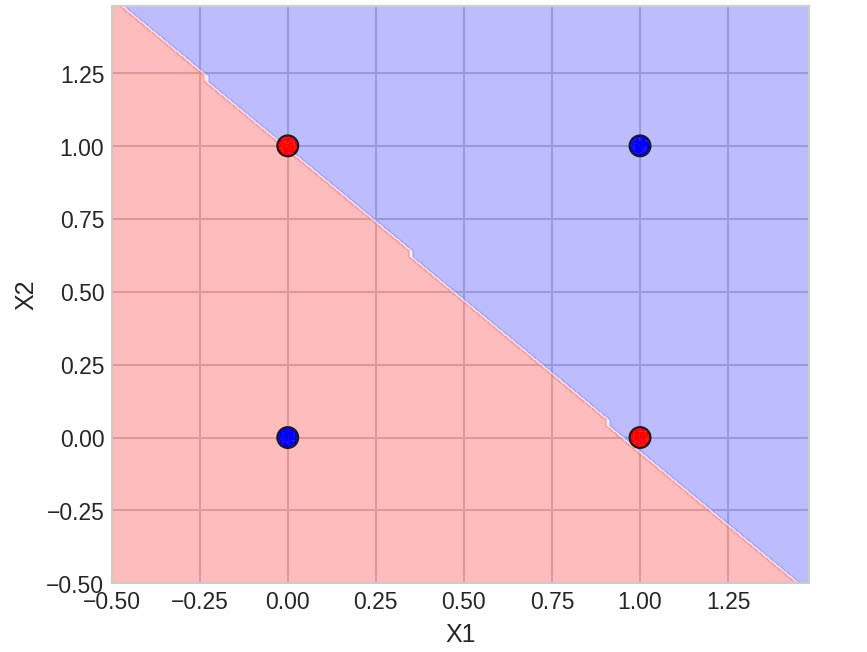
\includegraphics[width=0.65\textwidth]{40.jpg}
    \caption{Perceptron trên bài toán XOR (Không thể phân tách)}
    \label{fig:perceptron_xor}
    \vspace{-0.2cm}
\end{figure}

\section{Đánh giá kết quả cài đặt thuật toán MLP}
Nhóm đã cài đặt thành công Mạng nơ-ron nhiều lớp (MLP) hoàn toàn bằng NumPy, không sử dụng các framework học sâu như TensorFlow hay PyTorch. Mô hình được thiết kế linh hoạt thông qua tham số \texttt{layer\_sizes}, cho phép dễ dàng thay đổi số lượng lớp ẩn và số nơ-ron của từng lớp.

Quá trình Forward Propagation được triển khai bằng phép nhân ma trận, hỗ trợ các hàm kích hoạt Sigmoid và ReLU, đồng thời tự động lựa chọn Sigmoid hoặc Softmax ở lớp đầu ra kết hợp với Cross-Entropy Loss phù hợp với từng bài toán. Các giá trị trung gian được lưu lại để phục vụ cho quá trình lan truyền ngược.

Đối với Backward Propagation, nhóm đã cài đặt thành công thuật toán dựa trên quy tắc đạo hàm dây chuyền (Chain Rule) để tính gradient của trọng số và bias. Quá trình lan truyền sai số giữa các lớp được thực hiện chính xác bằng các phép toán ma trận NumPy. Kết quả thực nghiệm cho thấy thuật toán hoạt động ổn định, các trọng số được cập nhật chính xác thông qua Gradient Descent.

\begin{figure}[H]
    \centering
    \vspace{-0.3cm}
    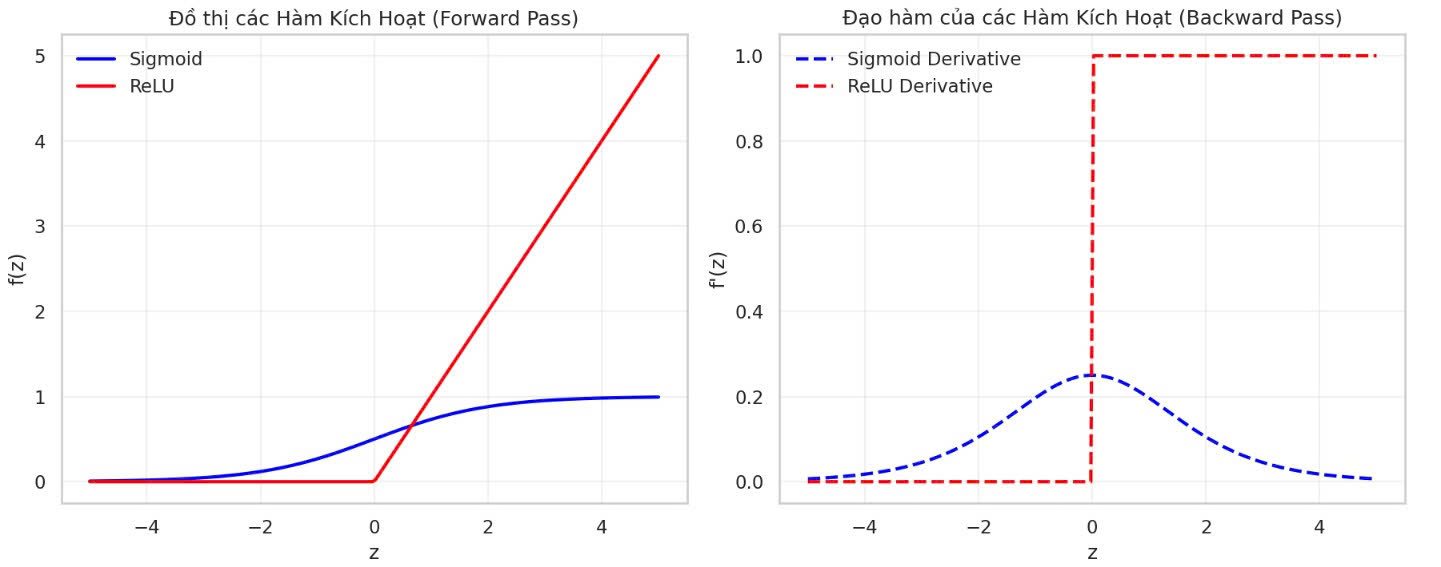
\includegraphics[width=0.85\textwidth]{41.jpg}
    \caption{Đồ thị các Hàm Kích Hoạt và Đạo hàm tương ứng}
    \label{fig:activation_functions}
    \vspace{-0.2cm}
\end{figure}

\section{Đánh giá trên bài toán XOR}
Đối với bài toán XOR, mạng MLP được cấu hình theo kiến trúc 2 Input – 4 Hidden – 1 Output và sử dụng hai hàm kích hoạt Sigmoid và ReLU để so sánh hiệu quả huấn luyện.

Kết quả thực nghiệm cho thấy mô hình MLP hội tụ thành công và phân loại chính xác 100\% các mẫu dữ liệu XOR, khắc phục hoàn toàn hạn chế của Perceptron một lớp. Biểu đồ Decision Boundary cho thấy mạng đã học được ranh giới quyết định phi tuyến. Đồng thời, đồ thị Loss theo Epoch cho thấy ReLU hội tụ nhanh hơn Sigmoid.

\begin{figure}[H]
    \centering
    \vspace{-0.3cm}
    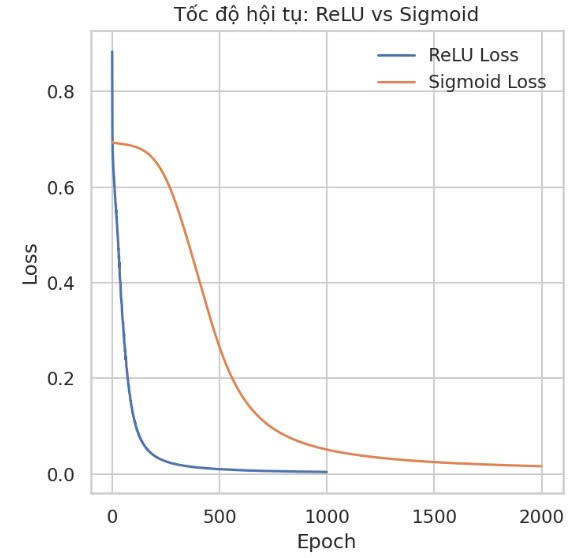
\includegraphics[width=0.7\textwidth]{42.jpg} \\[0.2cm]
    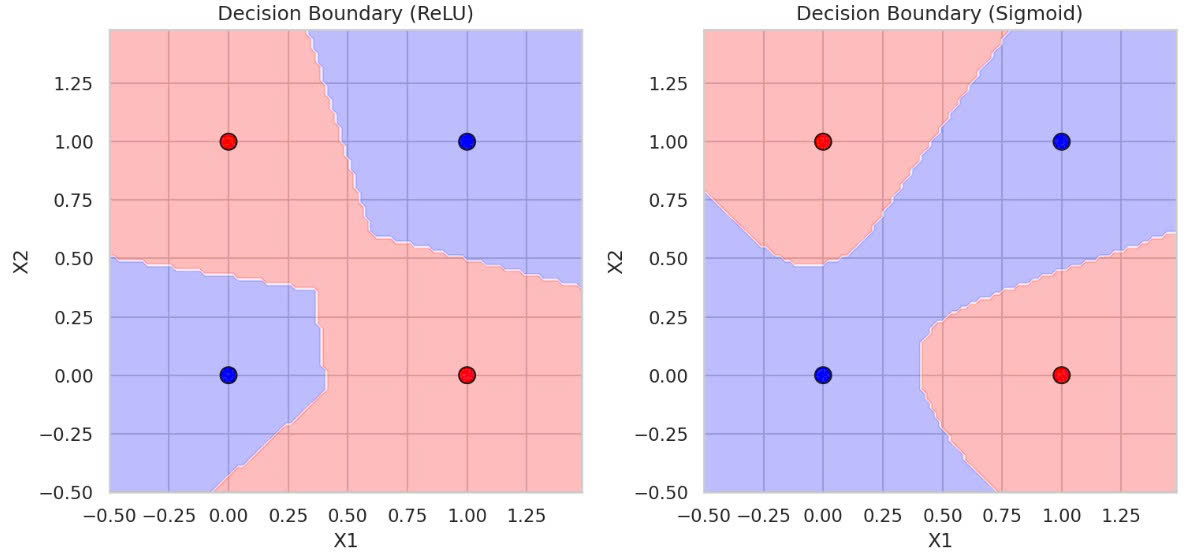
\includegraphics[width=0.7\textwidth]{43.jpg}
    \caption{Tốc độ hội tụ và ranh giới quyết định của MLP trên bài toán XOR}
    \label{fig:mlp_xor}
    \vspace{-0.2cm}
\end{figure}

\section{Đánh giá trên tập dữ liệu Iris}
Trước khi huấn luyện, dữ liệu Iris được chuẩn hóa bằng StandardScaler, chuyển đổi nhãn sang One-hot Encoding và chia theo tỷ lệ 80\% dữ liệu huấn luyện và 20\% dữ liệu kiểm tra. Mô hình được cấu hình theo kiến trúc 4 Input – 8 Hidden – 3 Output, sử dụng ReLU cho lớp ẩn, Softmax cho lớp đầu ra và Learning Rate = 0.1.

Kết quả huấn luyện cho thấy Train Loss và Validation Loss giảm đều và hội tụ sau khoảng 600 epochs. Khi đánh giá trên tập kiểm tra, mô hình đạt độ chính xác từ 96\% đến 100\%. 

\begin{figure}[H]
    \centering
    \vspace{-0.3cm}
    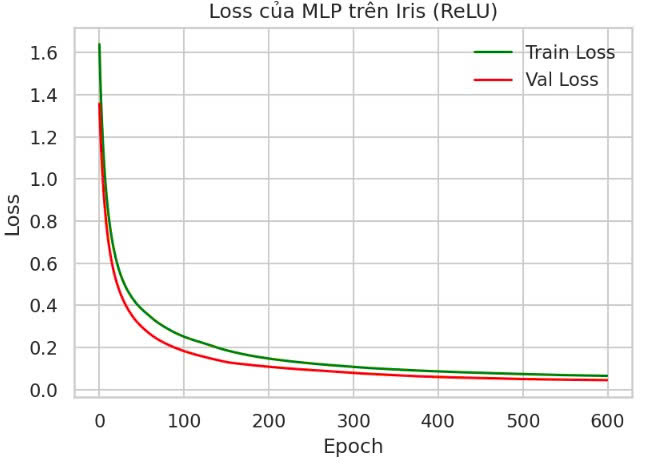
\includegraphics[width=0.85\textwidth]{44.jpg}
    \caption{Loss của MLP trên tập dữ liệu Iris (ReLU)}
    \label{fig:loss_iris}
    \vspace{-0.2cm}
\end{figure}


\chapter{THỰC NGHIỆM MỞ RỘNG}

\section{Đánh giá hiệu quả của thuật toán tối ưu SGD với Momentum}
Nhóm tiến hành huấn luyện hai mô hình MLP trên tập dữ liệu Iris, sử dụng lần lượt SGD và SGD with Momentum ($\beta=0.9$) với cùng cấu hình và số epoch để đánh giá hiệu quả của thuật toán tối ưu.

Kết quả thực nghiệm cho thấy SGD with Momentum có tốc độ hội tụ vượt trội. Đường Loss giảm nhanh và đạt mức khoảng $0.05$ chỉ sau gần 100 epochs, trong khi SGD vẫn còn ở mức khoảng $0.18$ sau 300 epochs. Điều này cho thấy Momentum giúp mô hình tìm đến điểm tối ưu nhanh hơn.

\begin{figure}[H]
    \centering
    \vspace{-0.3cm}
    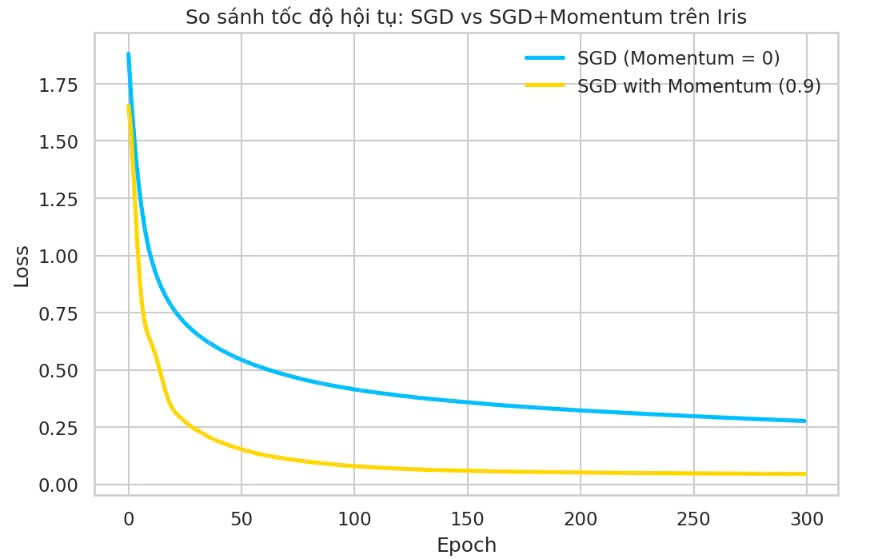
\includegraphics[width=0.75\textwidth]{45.jpg}
    \caption{So sánh tốc độ hội tụ: SGD vs SGD+Momentum trên Iris}
    \label{fig:sgd_momentum}
    \vspace{-0.2cm}
\end{figure}

\section{Ảnh hưởng của số lượng lớp ẩn (Hidden Layers)}
Nhóm tiến hành huấn luyện ba kiến trúc MLP trên tập dữ liệu Iris trong 500 epochs:
\begin{itemize}
    \item 1 lớp ẩn: [4–32–3]
    \item 2 lớp ẩn: [4–32–16–3]
    \item 3 lớp ẩn: [4–32–16–8–3]
\end{itemize}

\textbf{Kết quả thực nghiệm:}
\begin{itemize}
    \item \textbf{Mô hình 1 lớp ẩn:} Train Loss và Validation Loss giảm đều nhưng hội tụ chậm, đạt khoảng 0.06 sau gần 500 epochs.
    \item \textbf{Mô hình 2 lớp ẩn:} Hội tụ nhanh nhất, cả Train Loss và Validation Loss giảm mạnh và đạt khoảng 0.04 chỉ sau 150–200 epochs.
    \item \textbf{Mô hình 3 lớp ẩn:} Loss tiếp tục giảm đến khoảng 0.02, tuy nhiên tốc độ và độ chính xác chỉ cải thiện rất ít so với mô hình 2 lớp ẩn, trong khi số lượng tham số tăng đáng kể.
\end{itemize}

Kiến trúc [4–32–16–3] là lựa chọn tối ưu cho bài toán phân loại Iris, giúp mô hình học nhanh, ổn định và có khả năng tổng quát hóa tốt.

\begin{figure}[H]
    \centering
    \vspace{-0.3cm}
    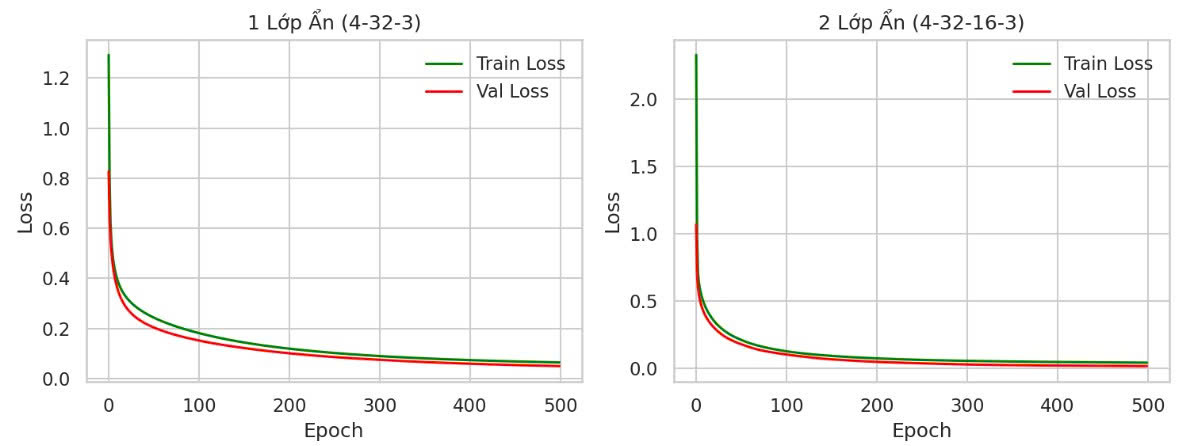
\includegraphics[width=0.7\textwidth]{46.jpg} \\[0.2cm]
    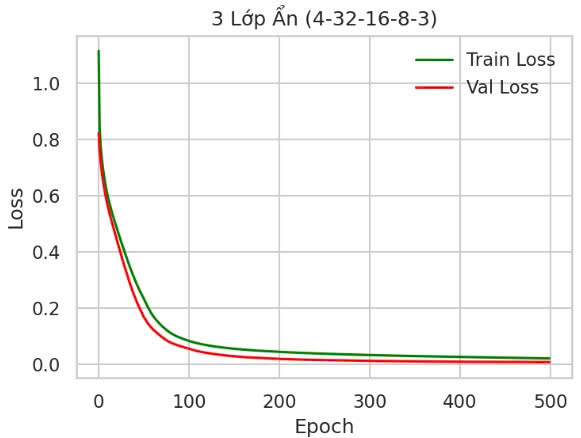
\includegraphics[width=0.7\textwidth]{47.jpg}
    \caption{Ảnh hưởng của số lượng lớp ẩn đến quá trình huấn luyện}
    \label{fig:hidden_layers}
    \vspace{-0.2cm}
\end{figure}

\section{Đánh giá hiệu quả của L2 Regularization}
Để đánh giá khả năng chống overfitting, nhóm sử dụng mô hình MLP có cấu trúc lớn (4–64–32–3) và chỉ huấn luyện trên 30 mẫu dữ liệu trong 800 epochs. Thực nghiệm được so sánh giữa hai trường hợp không sử dụng L2 ($\lambda=0$) và có sử dụng L2 ($\lambda=0.15$).

Kết quả thực nghiệm: Khi không sử dụng L2, Train Loss giảm rất nhanh về gần 0 trong khi Validation Loss dừng ở mức cao (khoảng 0.2), cho thấy mô hình bị overfitting. Ngược lại, khi áp dụng L2 Regularization, Train Loss giảm chậm hơn nhưng ổn định, đồng thời Validation Loss tiếp tục giảm xuống khoảng 0.1, khoảng cách giữa Train Loss và Validation Loss được thu hẹp đáng kể.

\begin{figure}[H]
    \centering
    \vspace{-0.3cm}
    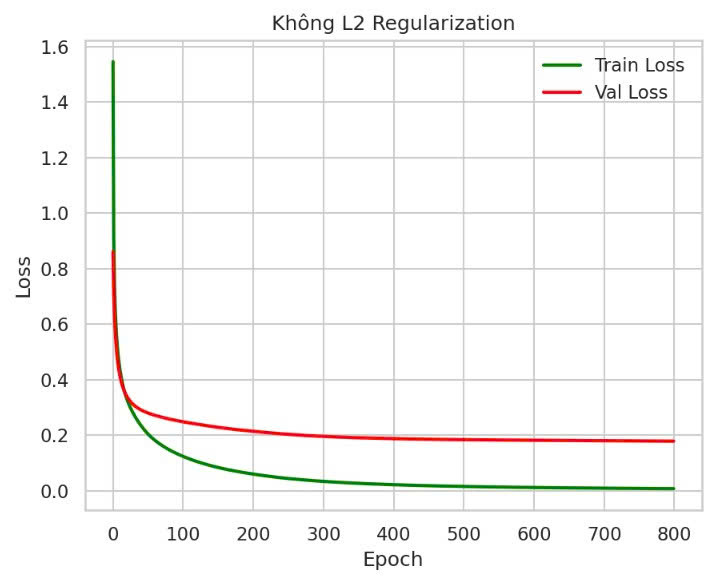
\includegraphics[width=0.75\textwidth]{49.jpg} \\[0.2cm]
    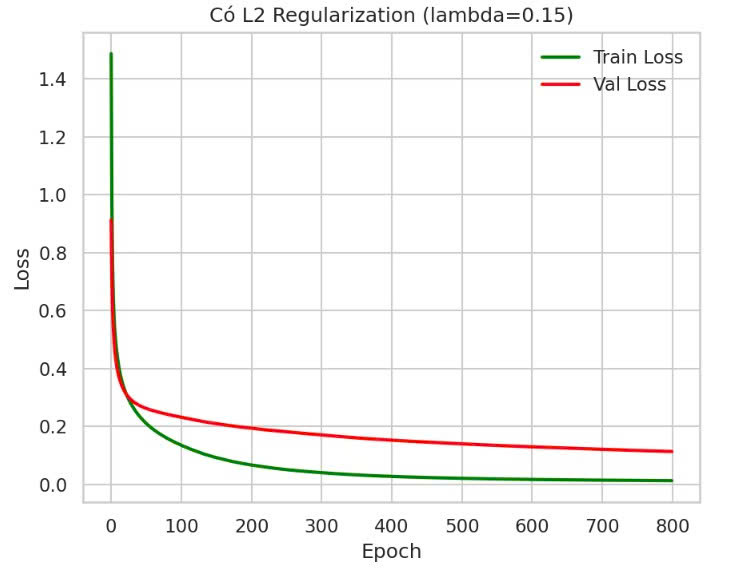
\includegraphics[width=0.75\textwidth]{50.jpg}
    \caption{Đánh giá hiệu quả chống Overfitting của L2 Regularization}
    \label{fig:l2_regularization}
    \vspace{-0.2cm}
\end{figure}

\chapter{DỮ LIỆU VÀ MÔI TRƯỜNG XỬ LÝ}

\section{Tập dữ liệu}
Đề tài sử dụng hai tập dữ liệu để kiểm thử và đánh giá mô hình:
\begin{itemize}
    \item \textbf{Tập dữ liệu XOR:} Gồm 4 mẫu nhị phân $(0,0) \rightarrow 0, (0,1) \rightarrow 1, (1,0) \rightarrow 1, (1,1) \rightarrow 0$. Bộ dữ liệu này được sử dụng để kiểm chứng giới hạn của Perceptron và khả năng giải quyết bài toán phi tuyến của mạng MLP.
    \item \textbf{Tập dữ liệu Iris:} Bộ dữ liệu gồm 150 mẫu, thuộc 3 loài hoa Iris, mỗi mẫu có 4 đặc trưng. Dữ liệu được chuẩn hóa bằng StandardScaler, nhãn được mã hóa One-Hot Encoding, sau đó chia thành tập huấn luyện (80\%) và kiểm tra (20\%).
\end{itemize}

\section{Môi trường và thư viện}
Các thực nghiệm được thực hiện trên Python 3.13 trong Google Colab (Visual Studio Code).
Các thư viện sử dụng gồm:
\begin{itemize}
    \item \textbf{NumPy:} Cài đặt toàn bộ mô hình Perceptron, MLP, Forward Propagation, Backpropagation, SGD, Momentum và L2 Regularization.
    \item \textbf{Matplotlib, Seaborn:} Trực quan hóa đồ thị Loss, Decision Boundary và Confusion Matrix.
    \item \textbf{Scikit-learn:} Hỗ trợ tải dữ liệu Iris, chuẩn hóa dữ liệu, chia tập huấn luyện/kiểm tra và đánh giá mô hình.
\end{itemize}

\chapter{KẾT LUẬN}

\section{Những kết quả đã đạt được}
Trong đề tài này, nhóm đã hoàn thành xuất sắc các mục tiêu đề ra ban đầu, bao gồm:
\begin{itemize}
    \item \textbf{Cài đặt thành công mô hình từ đầu (scratch):} Xây dựng thành công mô hình Perceptron và Mạng nơ-ron nhiều lớp (MLP) hoàn toàn bằng thư viện toán học NumPy mà không phụ thuộc vào các framework học sâu có sẵn (như PyTorch hay TensorFlow).
    \item \textbf{Am hiểu sâu sắc cơ sở toán học:} Áp dụng chính xác các công thức toán học về Lan truyền thuận (Forward Propagation) và Lan truyền ngược (Backpropagation) sử dụng quy tắc đạo hàm dây chuyền (Chain Rule) trên hệ thống ma trận (Batch Matrix).
    \item \textbf{Phát triển các thuật toán tối ưu tiên tiến:} Không chỉ dừng lại ở thuật toán cập nhật cơ bản (SGD), nhóm đã tự cài đặt thành công thuật toán tối ưu có gia tốc (SGD with Momentum) giúp tăng tốc độ hội tụ, và thuật toán điều chuẩn (L2 Regularization / Weight Decay) giúp giảm thiểu mạnh mẽ hiện tượng Overfitting.
    \item \textbf{Thực nghiệm và trực quan hóa chi tiết:} Đánh giá toàn diện trên cả dữ liệu phi tuyến (XOR) và dữ liệu thực tế nhiều đặc trưng (Iris). Trực quan hóa và phân tích chi tiết các đồ thị hàm mất mát, ranh giới quyết định (Decision Boundary), qua đó minh chứng khoa học được ưu/nhược điểm của từng cấu hình mạng.
\end{itemize}

\section{Những mặt còn hạn chế}
Mặc dù đã đạt được nhiều kết quả tích cực, mô hình và đề tài vẫn còn một số hạn chế nhất định:
\begin{itemize}
    \item \textbf{Hiệu suất tính toán:} Việc tính toán ma trận hoàn toàn bằng CPU thông qua NumPy sẽ gặp trở ngại về tốc độ nếu mở rộng sang các tập dữ liệu kích thước lớn (như xử lý ảnh, văn bản), do chưa tận dụng được sức mạnh tính toán song song của GPU (CUDA).
    \item \textbf{Thuật toán tối ưu:} Đề tài mới chỉ áp dụng SGD with Momentum. Trong thực tế, các kiến trúc Deep Learning hiện đại thường yêu cầu các thuật toán tối ưu tự thích ứng (Adaptive Learning Rate) như Adam hay RMSprop để hội tụ tốt hơn trên các không gian hao phí phức tạp.
    \item \textbf{Cơ chế dừng sớm (Early Stopping):} Quá trình huấn luyện hiện tại chạy cố định theo số vòng lặp (Epochs) được định trước. Nếu mô hình đã tìm được điểm tối ưu cục bộ sớm, việc tiếp tục tính toán gây lãng phí tài nguyên.
\end{itemize}

\section{Hướng phát triển trong tương lai}
Từ những hạn chế trên, nhóm đề xuất các hướng phát triển tiếp theo cho đề tài:
\begin{itemize}
    \item \textbf{Tích hợp thuật toán Adam:} Cài đặt bổ sung thuật toán Adam (Adaptive Moment Estimation) để tự động điều chỉnh tốc độ học cho từng tham số mạng, giúp quá trình hội tụ nhanh, ổn định và ít phụ thuộc vào việc điều chỉnh siêu tham số thủ công.
    \item \textbf{Phát triển cơ chế Early Stopping:} Lập trình module theo dõi độ đo trên tập Validation, tự động ngắt quá trình huấn luyện khi Validation Loss có dấu hiệu tăng trở lại (dấu hiệu của Overfitting), giúp tiết kiệm thời gian và tài nguyên.
    \item \textbf{Mở rộng dữ liệu và kiến trúc:} Thử nghiệm mô hình tự xây dựng trên các tập dữ liệu lớn và phức tạp hơn như nhận dạng chữ số viết tay (MNIST) hoặc dữ liệu ảnh màu (CIFAR-10) để kiểm tra tính bền vững của mã nguồn.
    \item \textbf{Đóng gói thành thư viện độc lập:} Tái cấu trúc mã nguồn theo hướng đối tượng (OOP) sâu hơn, đóng gói thành một thư viện Micro-DeepLearning với các API dễ gọi (tương tự như \texttt{torch.nn.Sequential} của PyTorch).
\end{itemize}

\begin{center}
    \vspace{1cm}
    \textbf{--- HẾT ---}
\end{center}

\end{document}